\documentclass[lettersize,journal]{IEEEtran}
\usepackage{amsmath,amsfonts}
\usepackage{algorithmic}
\usepackage{algorithm}
\usepackage{array}
\usepackage[caption=false,font=normalsize,labelfont=sf,textfont=sf]{subfig}
\usepackage{textcomp}
\usepackage{stfloats}
\usepackage{url}
\usepackage{verbatim}
\usepackage{graphicx}
\usepackage{cite}
\hyphenation{op-tical net-works semi-conduc-tor IEEE-Xplore}

\begin{document}

\title{NEURAL NETWORKS - DEEP LEARNING \\ FIRST ASSIGNMENT}

\author{Dimitrios Diakoloukas 10642, Electrical and Computer Engineering,~\IEEEmembership {AUTH, Student}

\thanks{}
\thanks{}}

% The paper headers
\markboth{FIRST ASSIGNMENT NEURAL NETWORKS - DEEP LEARNING, 
 November~2024}%
{Shell \MakeLowercase{\textit{et al.}}: A Sample Article Using IEEEtran.cls for IEEE Journals}

\maketitle

\begin{abstract}
This project implements and compares three models—k-Nearest Neighbor (k-NN), Convolutional Neural Network (CNN), and Multi-Layer Perceptron (MLP)—for multi-class classification on the CIFAR-10 dataset. Each model’s performance was evaluated based on accuracy, using both training and testing data. The CNN demonstrated superior feature extraction and classification capabilities, while the MLP provided insight into performance with fully connected layers. The k-NN model served as a baseline comparison. Results highlight each model's strengths and limitations, offering a detailed analysis of their effectiveness on CIFAR-10.
\end{abstract}

\section{Introduction}
\IEEEPARstart{I}{mage} classification is an essential task in computer vision, used in areas like autonomous driving and facial recognition. This project tests variations of three models—k-Nearest Neighbor (k-NN), Convolutional Neural Network (CNN), and Multi-Layer Perceptron (MLP)—on the CIFAR-10 dataset, which has 60,000 images in 10 classes.

The k-NN models serve as a simple, distance-based baseline. The CNNs use convolutional layers to capture patterns in images, making them especially effective for this task. The MLPs, a fully connected network, show how traditional neural networks handle image classification.

Each model’s accuracy is evaluated on CIFAR-10 to compare their strengths and weaknesses, highlighting the advantages of more advanced models like CNNs over simpler ones like k-NN.

\section{Data Loading and Preprocessing}

This section explains how Iloaded the CIFAR-10 dataset and prepared it so it could be used with the k-Nearest Neighbor (k-NN) algorithm.

\subsection{\textbf{Loading CIFAR-10 Data}}
The CIFAR-10 dataset contains 60,000 small color images (32x32 pixels) across 10 different classes. There are 50,000 images for training and 10,000 images for testing. Each image is stored as a set of pixel values, and the data is divided into multiple files.

I used the following steps to load the data:
\begin{itemize}
    \item \textbf{Unpacking Data Files:} The training data is stored in five files, each containing 10,000 images. I created a helper function called unpickle to open each file and load the data inside.
    \item \textbf{Combining Training Files:} I combined the data from all five training files into one large set. This gave us a total of 50,000 images for training. I did the same for the labels, so each image has a label showing which class it belongs to.
    \item \textbf{Loading Test Data:} The test data is stored in a separate file. I loaded this file in the same way to get 10,000 test images and their labels.
\end{itemize}

\subsection{\textbf{Data Preprocessing}}
After loading the data, I prepared it for use with machine learning by following these steps:

\begin{itemize}
    \item \textbf{Reshaping Images:} Each image was originally stored as a long row of numbers (a flat array). I reshaped these numbers back into the original 32x32 size with 3 color channels (Red, Green, and Blue).
    \item \textbf{Normalizing Pixel Values:} The pixel values in each image were originally between 0 and 255. To make the data easier to work with, I scaled these values to be between 0 and 1 by dividing each value by 255. This helps the model perform better and faster.
\end{itemize}

The final output of our data loading and preprocessing is:
\begin{itemize}
    \item \texttt{x\_train}: A set of 50,000 training images, each with shape (32, 32, 3) and pixel values between 0 and 1.
    \item \texttt{y\_train}: A set of 50,000 labels for the training images.
    \item \texttt{x\_test}: A set of 10,000 test images, also with shape (32, 32, 3) and pixel values between 0 and 1.
    \item \texttt{y\_test}: A set of 10,000 labels for the test images.
\end{itemize}
\vspace{0.3cm}
This data is now ready to be used in our CNN and MLP algorithms as well as the k-NN algorithm, making it easy to classify each image based on its pixel values.


\section{The k-Nearest Neighbor (k-NN) Algorithm}

The k-Nearest Neighbor (k-NN) algorithm is a simple, method used for classification tasks. In classification, the algorithm works by identifying the "k" closest data points (or neighbors) to a given input and predicting the class based on these neighbors.

The steps of the k-NN algorithm are as follows:

\begin{enumerate}
    \item \textbf{Choosing the Number of Neighbors (k):} The user selects the number of nearest neighbors (k) that will be used to make the prediction. A small k value can make the model more sensitive to noise and a larger k value may make it too generalized.
    
    \item \textbf{Calculating Distance:} For a new data point, the algorithm calculates the distance between this point and all points in the training data. Common distance metrics include Euclidean distance, Manhattan distance, and Minkowski distance, with Euclidean distance being the most widely used in k-NN classification and the one I used in our implementations later on.
    
    \item \textbf{Finding the k Nearest Neighbors:} After calculating the distances, the algorithm identifies the "k" closest data points in the training set.
    
    \item \textbf{Assigning the Class Label:} The algorithm assigns the new data point to the class that appears most frequently among the k neighbors. For example, if $k=5$ and three neighbors are in class A while two are in class B, the new point is classified as class A.
\end{enumerate}


\subsection{\textbf{Advantages and Disadvantages of k-NN}}

\textbf{Advantages:}
\begin{itemize}
    \item \textbf{}{Simplicity:} k-NN is easy to implement and understand.
    \item \textbf{No Training Phase:} Not complicated because the computation happens during prediction.
    \item \textbf{Flexibility:} Works well with various distance metrics (like Euclidean, Manhattan, etc) and can be adjusted for specific tasks by changing the value of k.
\end{itemize}

\textbf{Disadvantages:}
\begin{itemize}
    \item \textbf{Computational Cost:} Since k-NN requires calculating distances for all points in the training set, it can be slow and computationally expensive with large datasets. Since this is a major disadvantage I used only 2000 training examples in the implementation without PCA (Principal Component Analysis). In our implementation with PCA I used the entire CIFAR-10 dataset (60000 32x32 colour images in 10 classes) since PCA can reduce its dimensionality while keeping as much variation as possible making the k-NN algorithm operate quicker.
    \item \textbf{Sensitive to Scale:} k-NN needs preprocessing (like normalization) for better performance.
    \item \textbf{Sensitive to Imbalanced Data:} If one class has many more examples than others, k-NN might favor that class in its predictions.
\end{itemize}
\vspace{0.3cm}

That is why k-NN gave us worse accuracy results overall than the Convolutional Neural Network (CNN), and Multi-Layer Perceptron (MLP).
For this project though it provides a simple comparison to evaluate the effectiveness of more complex neural network models like CNN and MLP.

\subsection{\textbf{Approach of the Task}}

\textbf{1. Custom Implementation of k-NN Without PCA}

In this approach, I implemented k-NN from scratch, using Euclidean distance to measure similarity between points. Each image was flattened into a 1D vector, and I used a subset of 2000 samples for both training and testing to keep it manageable, as the algorithm was quite slow.

\begin{itemize}
    \item \textbf{Distance Calculation}: The distance between each test image and all training images is calculated.
    \item \textbf{Classification}: Each test image is labeled based on the most common label among its \( k \) nearest neighbors.
    \item \textbf{Nearest Centroid}: Ialso implemented a centroid-based classifier, which assigns each test image to the nearest class centroid.
    \item \textbf{Results}:
    \begin{enumerate}
        \item \textbf{k-NN with \( k = 1 \) Accuracy:} 0.244
        \item \textbf{k-NN with \( k = 3 \) Accuracy:} 0.255
        \item \textbf{Nearest Centroid Accuracy:} 0.271
    \end{enumerate}
\end{itemize}

\vspace{0.3cm}

\textbf{2. Custom Implementation of k-NN with PCA}

In this approach, Iused Principal Component Analysis (PCA) to reduce the data to 100 features, making the algorithm faster. Both k-NN and centroid classification were then applied to this simplified dataset.

\begin{itemize}
    \item \textbf{Dimensionality Reduction}: PCA was used to reduce each image to 100 features.
    \item \textbf{k-NN and Centroid Classification}: Both k-NN and nearest centroid classifiers were used on the reduced data.
    \item \textbf{Results}:
    \begin{enumerate}
        \item \textbf{k-NN with \( k = 1 \) Accuracy:} 0.3863
        \item \textbf{k-NN with \( k = 3 \) Accuracy:} 0.3893
        \item \textbf{Nearest Centroid Accuracy:} 0.2767
    \end{enumerate}
\end{itemize}

\vspace{0.3cm}

\textbf{3. Using sklearn Library for k-NN and Centroid Classifier with PCA}

In this approach, Iused the KNeighborsClassifier and NearestCentroid from sklearn. PCA was applied to reduce each image to 100 features, making it faster to process. The optimized classifiers from sklearn gave us an efficient and scalable implementation.

\begin{itemize}
    \item \textbf{Optimized Implementation}: KNeighborsClassifier and NearestCentroid offer fast, built-in methods for k-NN and centroid classification.
    \item \textbf{Parameter Tuning}: sklearn makes it easy to adjust settings like the number of neighbors \( k \).
    \item \textbf{Efficiency}: Using sklearn improved performance and sped up the calculations on large datasets.
    \item \textbf{Results}:
    \begin{enumerate}
        \item \textbf{k-NN with \( k = 1 \) Accuracy:} 0.3856
        \item \textbf{k-NN with \( k = 3 \) Accuracy:} 0.3691
        \item \textbf{Nearest Centroid Accuracy:} 0.2767
    \end{enumerate}
\end{itemize}

Each approach offers a unique perspective, from manual implementation to more efficient, library-based methods suitable for practical use and are widely known.

\section{MLP Models Approaches}
A Multilayer Perceptron (MLP) is a basic type of neural network used in deep learning. It is called a feedforward network because data moves in one direction, starting from the input layer, passing through hidden layers, and ending at the output layer. MLPs can learn to model complex patterns, making them useful for tasks like classifying data or predicting outcomes. In our case I have build 4 MLP models to make predictions in the CIFAR-10 dataset.

\subsection{\textbf{All approaches and implementations}}
\subsubsection{\textbf{Initial Approach: Single-Layer MLP for CIFAR-10}}
\paragraph{\textbf{Explanation of initial approach}}
To begin I implemented a simple MLP with a single hidden layer to classify images from the CIFAR-10 dataset. My aim was to evaluate the basic performance of an MLP architecture and identify its strengths and limitations before attempting some more complex models.

\paragraph{\textbf{Model Architecture}}

The implemented MLP model had the following structure:
\begin{itemize}
    \item \textbf{Input Layer:} The input layer flattened each 32x32x3 image into a vector of size 3072, making it suitable for processing by a fully connected layer.
    \item \textbf{Hidden Layer:} A single hidden layer with 128 neurons was used, applying the ReLU (Rectified Linear Unit) activation function to introduce non-linearity.
    \item \textbf{Dropout:} A dropout layer with a rate of 0.5 was added after the hidden layer to reduce overfitting by randomly deactivating 50\% of the neurons during training.
    \item \textbf{Output Layer:} The output layer consisted of 10 neurons (one for each class), using the softmax activation function to compute probabilities for each class.
\end{itemize}

The model was compiled with the Adam optimizer and the categorical crossentropy loss function, which are commonly used for classification tasks. The training process involved 20 epochs with a batch size of 128.

\paragraph{\textbf{Results}}
During training, I tracked the accuracy and loss for both the training and validation datasets. Figure 1 shows the model's accuracy and loss over the 20 epochs.

\begin{figure}[h!]
    \centering
    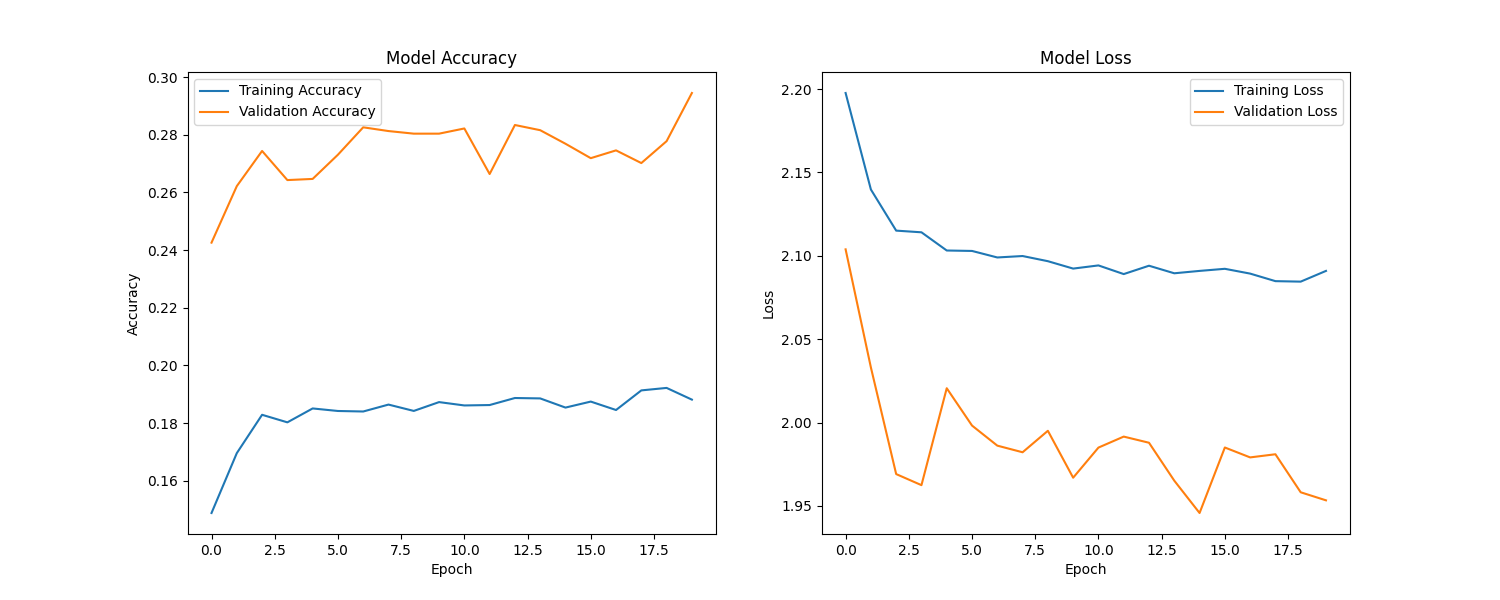
\includegraphics[width=0.5\textwidth]{training_history_MLP_onelayer.png}
    \caption{Training and Validation Accuracy and Loss for Single-Layer MLP.}
    \label{fig:onelayer_history}
\end{figure}

After training, the model achieved a test accuracy of around \textbf{\textit{0.3355}}

\paragraph{\textbf{Sample Predictions and Observations}}

To further evaluate the model, I visualized a selection of correctly and incorrectly classified images from the test set. Figure 2 displays 7 correct and 7 incorrect predictions. 

\begin{figure}[h!]
    \centering
    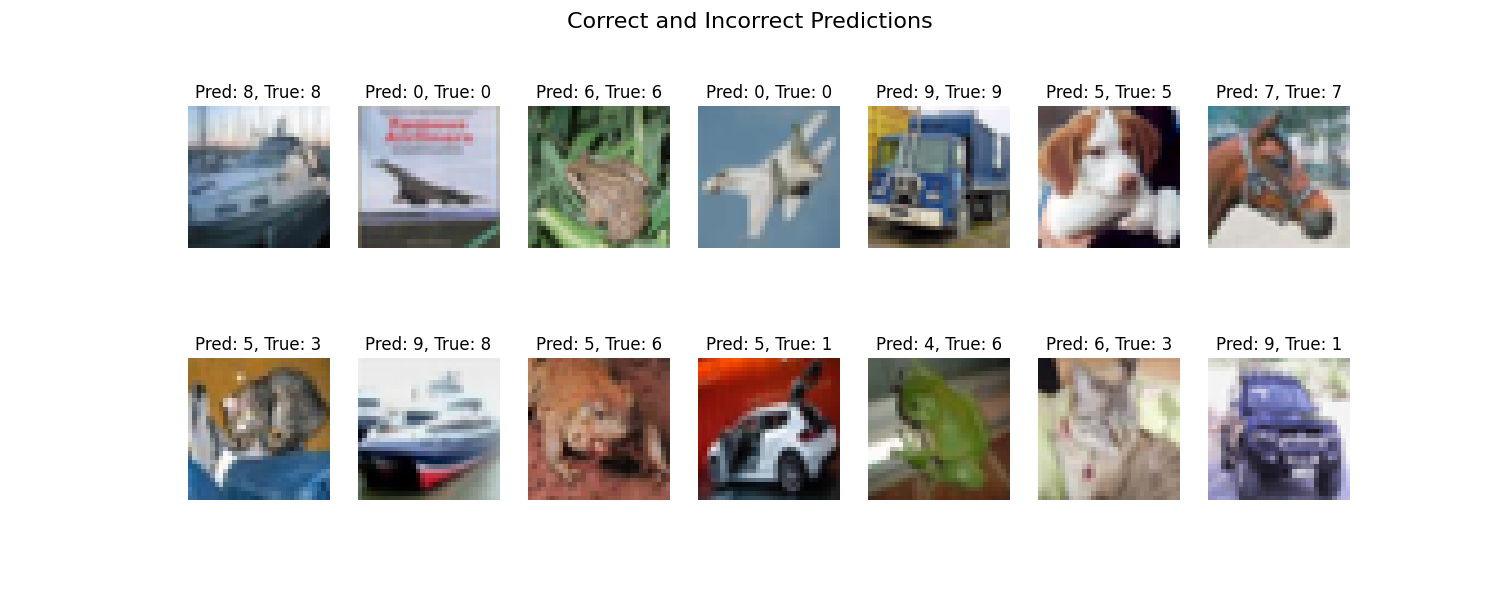
\includegraphics[width=0.5\textwidth]{sample_predictions_onelayer.png}
    \caption{Examples of Correct and Incorrect Predictions for Single-Layer MLP.}
    \label{fig:onelayer_predictions}
\end{figure}

Some of my key observations include:
\begin{itemize}
    \item The model performed well on simpler images with clear features but I think it might have struggled with some more complex images.
    \item The lack of multiple hidden layers reduces the ability to capture complex patterns.
    \item Overfitting might have happened to some extent by the dropout layer, but the model still seems to generalize well.
\end{itemize}

\subsubsection{\textbf{ MLP with more layers for CIFAR-10}}
\paragraph{\textbf{Model Explanation}}

Thw 

After trying a single-layer MLP, I built a more advanced model with two hidden layers to improve the performance. The goal was to help the network learn more complex patterns in the CIFAR-10 dataset and achieve better accuracy.

\paragraph{\textbf{Model Architecture}}

The improved MLP model was designed with the following layers:
\begin{itemize}
    \item \textbf{Input Layer:} The input layer flattened each 32x32x3 image into a vector of 3072 values.
    \item \textbf{First Hidden Layer:} This layer had 256 neurons and used the ReLU activation function to introduce non-linearity.
    \item \textbf{Dropout Layer:} A dropout rate of 0.3 was applied after the first hidden layer to reduce overfitting.
    \item \textbf{Second Hidden Layer:} This layer had 128 neurons and also used the ReLU activation function.
    \item \textbf{Dropout Layer:} Another dropout rate of 0.3 was applied after the second hidden layer for regularization.
    \item \textbf{Output Layer:} The output layer had 10 neurons, one for each class in CIFAR-10, and used the softmax activation function to calculate class probabilities.
\end{itemize}

The model was trained using the Adam optimizer and the categorical crossentropy loss function for 15 epochs with a batch size of 60.

\paragraph{\textbf{Results}}

During training, I tracked the accuracy and loss for both the training and validation datasets. Figure 3 shows the accuracy and loss for the model over the 15 epochs.

\begin{figure}[h!]
    \centering
    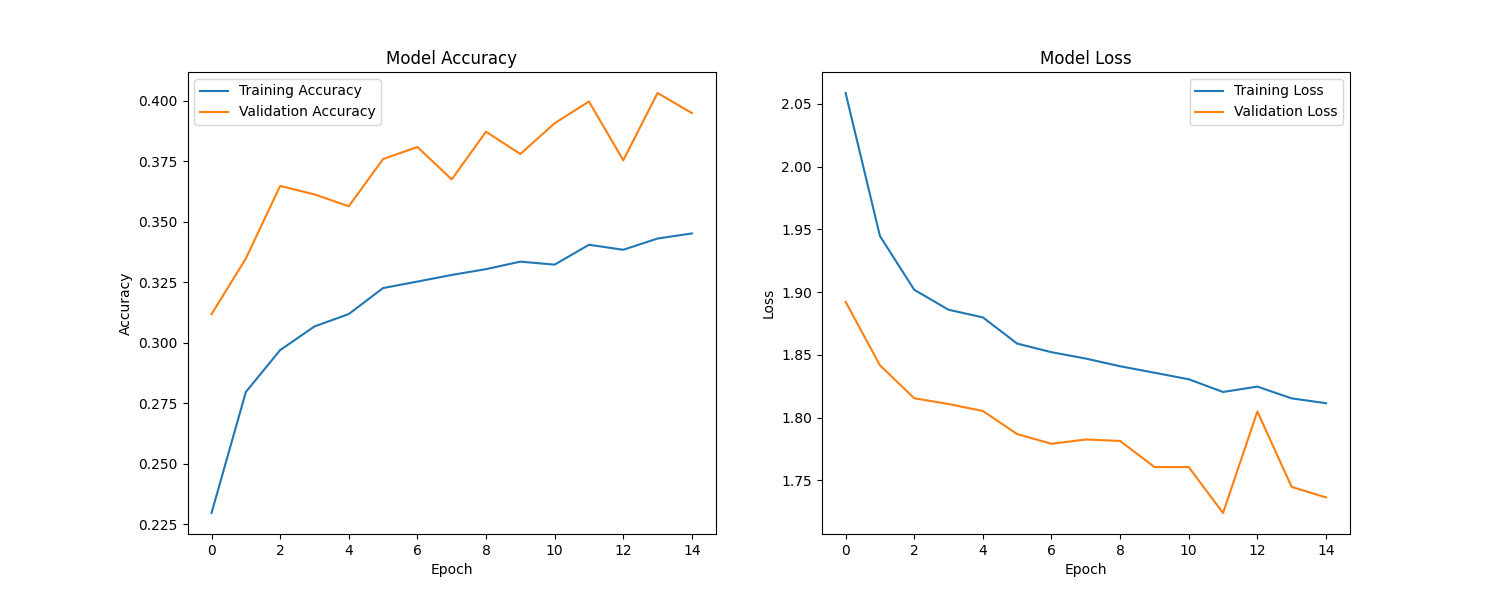
\includegraphics[width=0.5\textwidth]{training_history_MLP.png}
    \caption{Training and Validation Accuracy and Loss for Multi-Layer MLP.}
    \label{fig:mlp_training_history}
\end{figure}

The improved model performed better than the single-layer MLP. It achieved a test accuracy of around \textbf{0.4049}, which is a significant improvement.

\paragraph{\textbf{Sample Predictions}}

To check how well the model classified the images, I visualized some examples. Figure 4 shows 7 correctly classified and 7 incorrectly classified images from the test set.

\begin{figure}[h!]
    \centering
    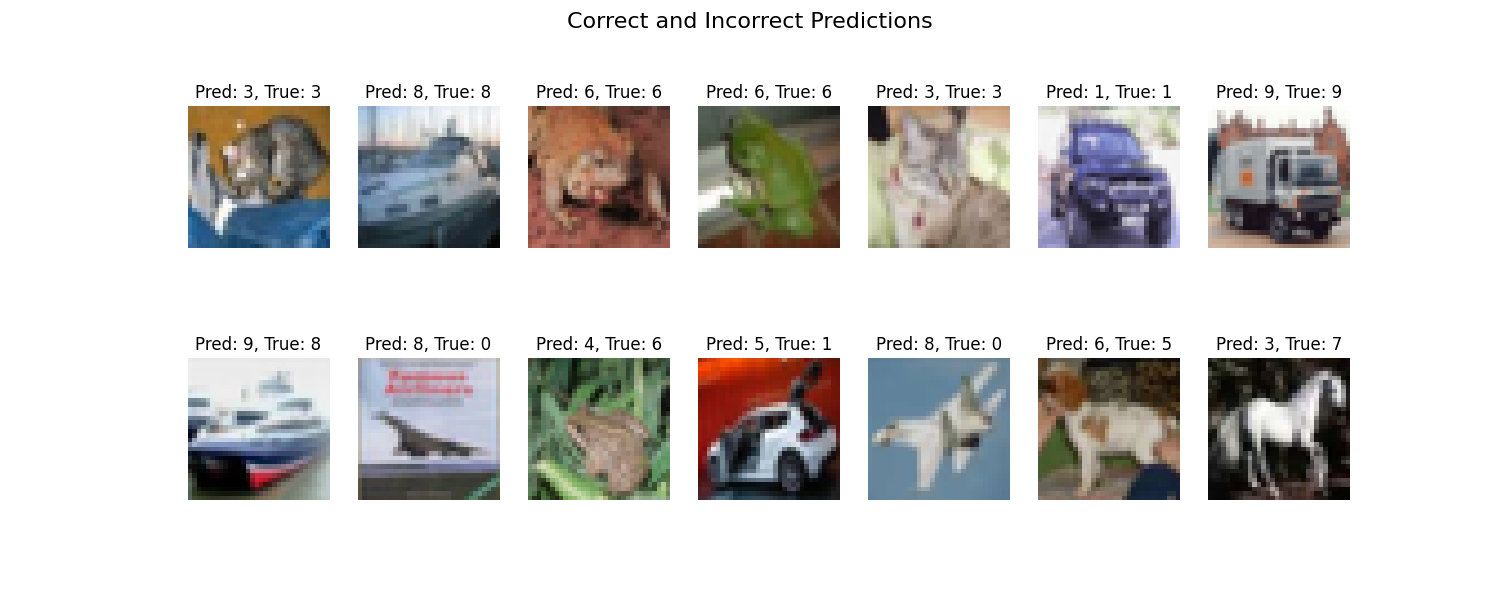
\includegraphics[width=0.5\textwidth]{sample_predictions_MLP.png}
    \caption{Examples of Correct and Incorrect Predictions for Multi-Layer MLP.}
    \label{fig:mlp_predictions}
\end{figure}

\paragraph{\textbf{Observations}}

The additional hidden layer and dropout made the model better at understanding the CIFAR-10 images. Some key takeaways:
\begin{itemize}
    \item The model learned more complex features, which improved its ability to classify the images correctly.
    \item Dropout layers reduced overfitting, as the validation accuracy stayed close to the training accuracy.
    \item However, the model still had difficulty with challenging images, which might need more advanced methods like convolutional layers to handle.
\end{itemize}

This improved MLP showed better performance than the simpler model and provided valuable insights for further improvements.

\subsubsection{\textbf{Best Approach: Advanced MLP for CIFAR-10}}
\paragraph{\textbf{Explanation of Best Approach}}

Building on the improvements in the multi-layer MLP, I designed an even more advanced MLP with three hidden layers, batch normalization, and higher dropout rates. To be more specific lets explain some of the terms I used. To begin with I used batch normalization as staded above. Batch normalization is a technique used to make training faster and more stable. It normalizes the inputs of each layer by adjusting and scaling them, ensuring the data has a mean of 0 and a standard deviation of 1 during training. This helps the network converge quicker and reduces sensitivity to initialization. Dropout on the other hand is a regularization method that randomly turns off a percentage of neurons during training. This prevents the model from relying too much on specific neurons, reducing overfitting and improving generalization to new data. The goal of this approach was to maximize the model's ability to classify the CIFAR-10 images by increasing its complexity and adding better regularization techniques.

\paragraph{\textbf{Model Architecture}}

The advanced MLP model was designed with the following layers:
\begin{itemize}
    \item \textbf{Input Layer:} The input layer flattened each 32x32x3 image into a vector of 3072 values.
    \item \textbf{First Hidden Layer:} This layer had 512 neurons and used the ReLU activation function. Batch normalization was applied to stabilize learning, followed by a dropout layer with a rate of 0.4 to reduce overfitting.
    \item \textbf{Second Hidden Layer:} This layer had 256 neurons, again with ReLU activation, batch normalization, and a dropout rate of 0.4.
    \item \textbf{Third Hidden Layer:} This layer had 128 neurons, ReLU activation, batch normalization, and a smaller dropout rate of 0.3.
    \item \textbf{Output Layer:} The final layer had 10 neurons, one for each class in CIFAR-10, and used the softmax activation function to calculate class probabilities.
\end{itemize}

The model was trained using the Adam optimizer with a learning rate of 0.001 and the categorical crossentropy loss function for 30 epochs with a batch size of 60.

\paragraph{\textbf{Results}}

The training and validation accuracy and loss were tracked throughout the 30 epochs. Figure 5 shows the accuracy and loss during training.

\begin{figure}[h!]
    \centering
    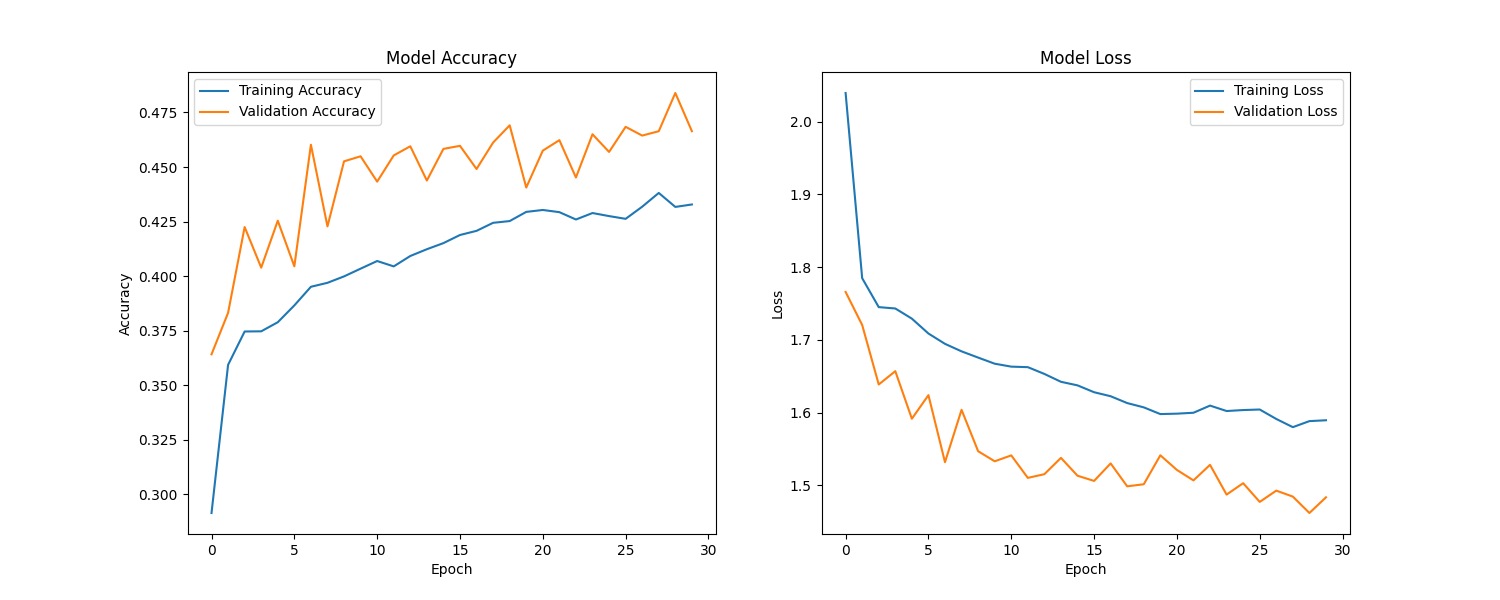
\includegraphics[width=0.5\textwidth]{training_history_MLP_BEST.png}
    \caption{Training and Validation Accuracy and Loss for Advanced Multi-Layer MLP.}
    \label{fig:mlp_best_training_history}
\end{figure}

The advanced model performed significantly better than the previous MLPs. It achieved a test accuracy of approximately \textbf{ 0.47439}, showing its ability to handle better the complexities of the CIFAR-10 dataset comparing it to the previous two models.

\paragraph{\textbf{Sample Predictions}}

To further evaluate the model, I visualized some examples of correctly and incorrectly classified images from the test set. Figure 5 displays 7 correct and 7 incorrect predictions.

\begin{figure}[h!]
    \centering
    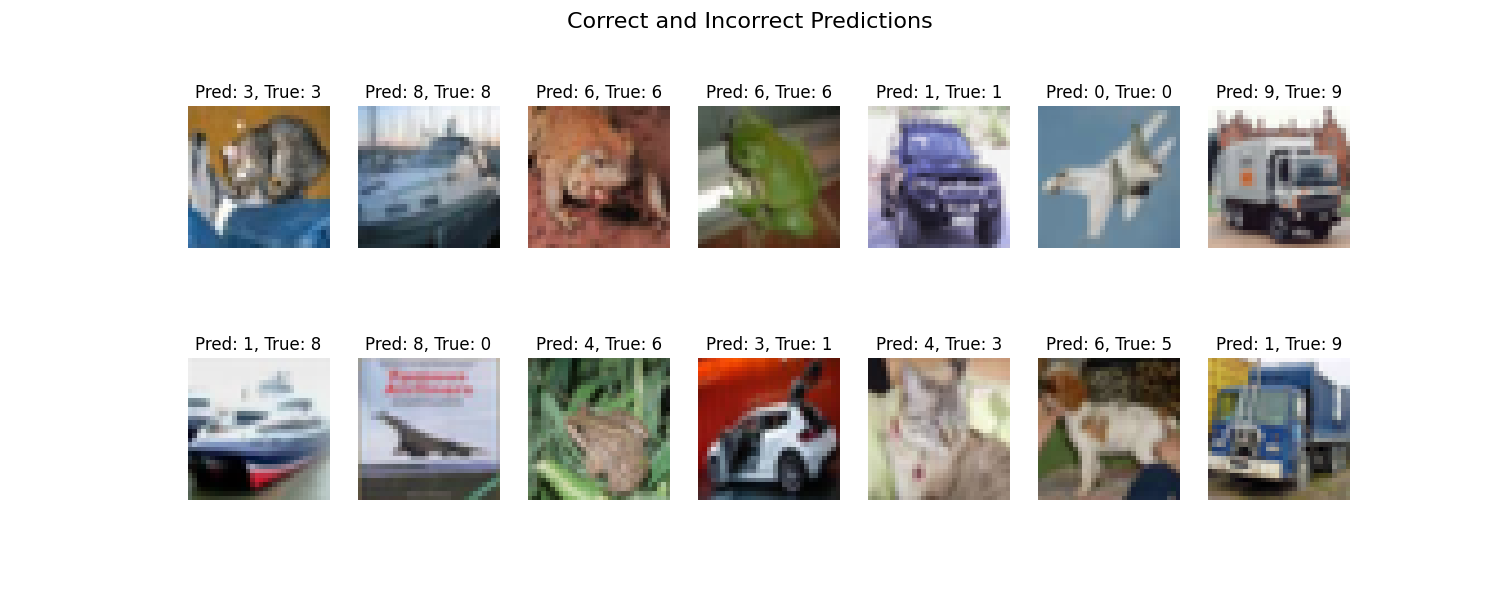
\includegraphics[width=0.5\textwidth]{sample_predictions_MLP_BEST.png}
    \caption{Examples of Correct and Incorrect Predictions for Advanced Multi-Layer MLP.}
    \label{fig:mlp_best_predictions}
\end{figure}

\paragraph{\textbf{Observations}}

The advanced MLP model achieved the best performance among all the approaches. Some of my takeaways include:
\begin{itemize}
    \item The increased number of neurons and hidden layers allowed the model to capture more complex patterns in the data.
    \item Batch normalization stabilized training and improved convergence, while dropout effectively reduced overfitting.
    \item Despite the improvements, the model occasionally struggled with challenging images which means that it could be even better with some convolutional layers in the implementation, and that might even produce better results.
\end{itemize}

This final keras based MLP approach used fully connected architectures combined with techniques like batch normalization and dropout.

\subsubsection{\textbf{Final Approach: Custom attempt on building MLP for CIFAR-10}}
\paragraph{\textbf{Explanation of Custom Approach}}
In this code I manually tried to implement a Multilayer Perceptron from scratch using NumPy. Unlike the Keras implementations, this code has the following features and some disadvantages but was created for experimenting purpose even though it has advantages over custom adjustments. So some important comparisons are the following:
\begin{itemize}
 \item \textbf{Control of the neural network implementation}:
    \begin{itemize}
        \item The custom code gives you full control over details like how weights are initialized, the learning rate, and how dropout is applied.
        \item Keras is easier to use but hides some of the details from the user.
    \end{itemize}
    
    \item \textbf{Optimization}:
    \begin{itemize}
        \item The custom code uses a simple method to update weights with a fixed learning rate.
        \item Keras uses more advanced optimizers like Adam, which adjust the learning rate automatically.
    \end{itemize}
    
    \item \textbf{Batch Normalization}:
    \begin{itemize}
        \item Keras includes batch normalization to make training faster and more stable.
        \item The custom implementation does not include this feature.
    \end{itemize}
    
    \item \textbf{Performance}:
    \begin{itemize}
        \item The custom code runs slower because NumPy doesn’t use GPUs.
        \item Keras is much faster because it can use GPUs for training.
    \end{itemize}
    
    \item \textbf{Flexibility}:
    \begin{itemize}
        \item The custom code lets you change everything, which is good for testing new ideas.
        \item Keras is better for quickly building and testing models.
    \end{itemize}
    
    \item \textbf{Visualization and Output}:
    \begin{itemize}
        \item Both codes create similar output, like accuracy and loss graphs and sample predictions.
        \item Keras does this automatically, but the custom code calculates it manually.
    \end{itemize}
\end{itemize}

Below I will now demonstrate the code implementation:
\begin{itemize}
    \item \textbf{Weight Initialization:} 
    The model starts by assigning random values (called weights) to each connection in the network. These weights are initialized using a method called He initialization, which makes sure the values are neither too large nor too small. This helps the model learn faster and avoid problems like vanishing gradients (when updates become very small). The specific method used (\textbf{He Initialization}) is shown down below:
\[
W \sim \mathcal{N}(0, \frac{2}{n_{\text{in}}})
\]
\begin{itemize}
    \item \( W \): The weight matrix being initialized.
    \item \( \mathcal{N}(0, \frac{2}{n_{\text{in}}}) \): A normal distribution with a mean of \( 0 \) and a variance of \( \frac{2}{n_{\text{in}}} \).
    \item \( n_{\text{in}} \): The number of input neurons (or the size of the previous layer).
\end{itemize}
This method ensures that the variance of activations remains stable across layers, which is especially useful for networks using the \textbf{ReLU activation function}:

    \item \textbf{My Layers and Architecture:}
    The MLP has the following structure:
    \begin{itemize}
        \item \textbf{Input Layer:} This layer takes the CIFAR-10 images, which are 32x32 pixels with 3 color channels. These images are flattened into a single row of 3072 numbers (32x32x3 = 3072 pixels).
        \item \textbf{Hidden Layers:} There are two hidden layers with 256 and 128 units (neurons). These layers use an activation function called ReLU (Rectified Linear Unit), which helps the network learn complex patterns by introducing non-linearity.
        \item \textbf{Output Layer:} The last layer has 10 units, one for each class in CIFAR-10. It uses the softmax activation function, which turns the output into probabilities for each class.
    \end{itemize}

    \item \textbf{Forward Pass:}
    The forward pass is the process where the input data is passed through the network, layer by layer, to produce predictions. A method called \texttt{dropout} is used during training to randomly turn off some neurons, which helps prevent overfitting (where the model performs well on training data but poorly on new data).

    \item \textbf{Backward Pass:}
    After the forward pass, the model compares its predictions with the true labels to calculate the error (loss). The backward pass then adjusts the weights in the network to minimize this error. This process, called backpropagation, uses the gradient descent method to update the weights step by step.

    \item \textbf{Loss Function:}
    The model uses a loss function called categorical crossentropy. This measures how different the predicted probabilities are from the actual labels. A smaller loss means the model is making better predictions.

    \item \textbf{My Training Loop:}
    The training loop is where the model learns:
    \begin{itemize}
        \item The data is mixed up randomly to keep it fair, and the model works on it in small parts called batches.
        \item For each batch, the model makes predictions (forward pass), calculates the loss, and adjusts the weights (backward pass).
        \item The training and validation performance (accuracy and loss) are recorded at every step.
    \end{itemize}
\end{itemize}

\paragraph{\textbf{Results and Visualizations}}

The results of training the custom MLP are shown in Figure 7. This figure displays how the accuracy and loss changed over 50 training epochs (iterations over the full dataset).

\begin{figure}[h!]
    \centering
    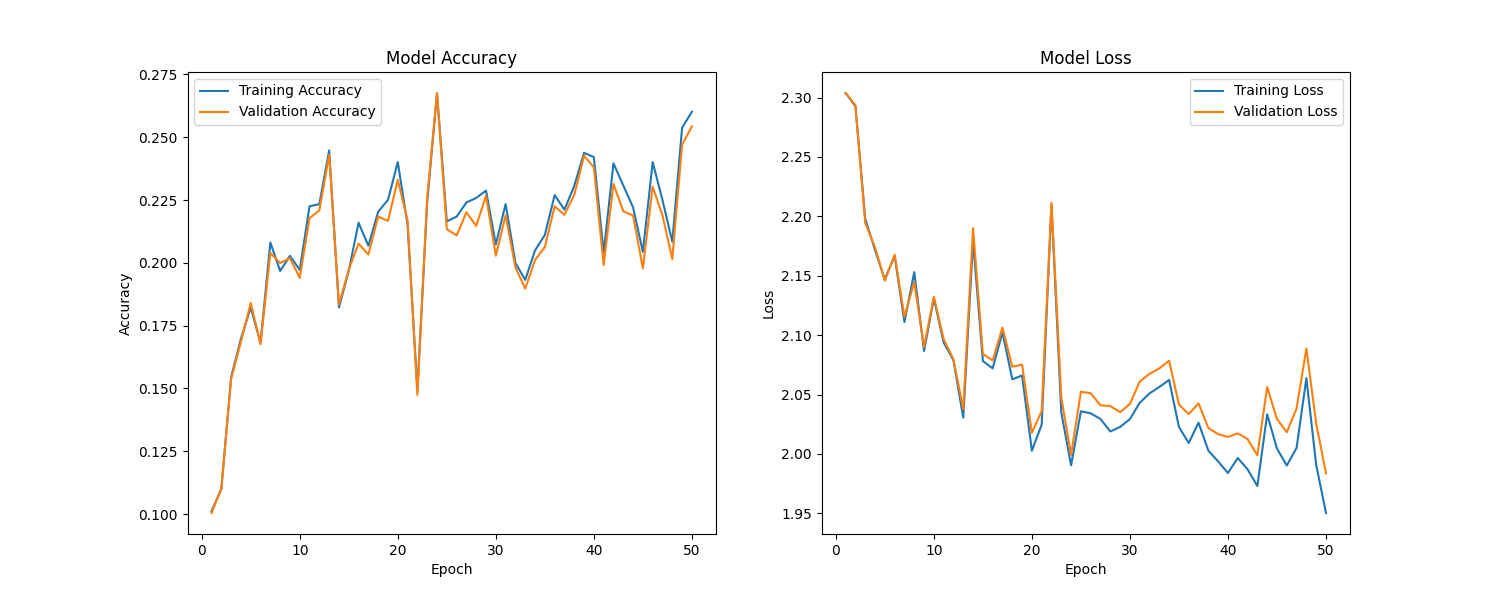
\includegraphics[width=0.5\textwidth]{training_history_custom_mlp.png}
    \caption{Training and Validation Accuracy and Loss for Custom MLP.}
    \label{fig:custom_training_history}
\end{figure}

After training, the model achieved a test accuracy of about \textbf{\textit{0.2543}} which means that the experimental model is still seriously struggling compared to the Keras ones as for its predictions. This is mostly due to reasons I have stated above like optimization, performance etc. To show you my model's performance, Figure 8 shows examples of images it classified correctly and incorrectly.

\begin{figure}[h!]
    \centering
    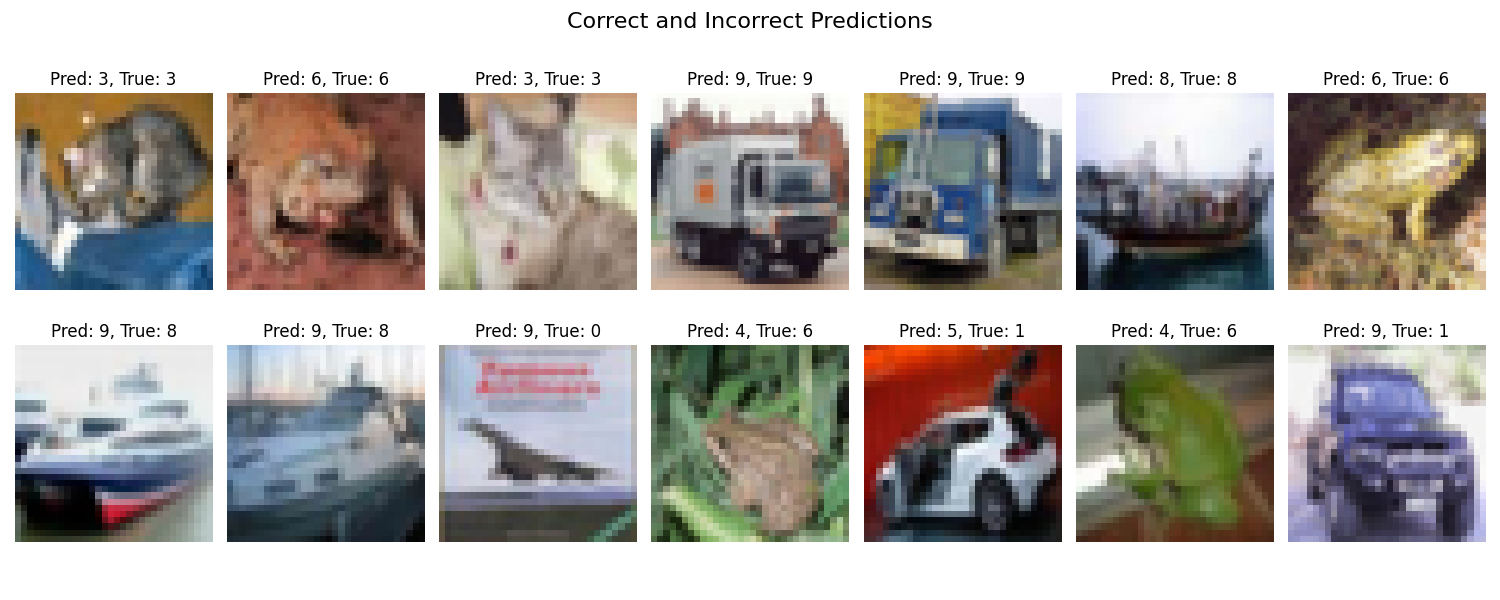
\includegraphics[width=0.5\textwidth]{sample_predictions_custom_mlp.png}
    \caption{Examples of Correct and Incorrect Predictions for Custom MLP.}
    \label{fig:custom_sample_predictions}
\end{figure}

\subsection{\textbf{Summary about MLP implementations}}
While MLP implementations of neural networks can be good and could most probably have better accuracy than the KNN algorithm there are a few other ways to achieve even better accuracy.
Later in my report paper I will show you some more advanced yet more commonly used neural network architectures for predictions in image datasets.

\section{CNN Model Approaches}
A Convolutional Neural Network (CNN) is a type of deep learning model that is especially effective for processing image data. Unlike MLPs, CNNs use convolutional layers to automatically learn spatial patterns in images, such as edges, textures, and objects. These networks are designed to handle the hierarchical structure of images, making them more efficient and accurate for image-related tasks. For this project, I developed 2 CNN models to classify images in the CIFAR-10 dataset and improve prediction accuracy. To be more specific I implemented one of them with data augmentations and one without and I will showcase and explain the differences later on in this section.

\subsection{\textbf{What is a CNN in a few words}}
\begin{enumerate}
    \item The input image is passed through convolutional layers, which extract features such as edges and textures.
    \item The pooling layers reduce the size of the feature maps, making the model faster and more robust.
    \item The extracted features are passed to fully connected layers for classification.
    \item The output layer provides probabilities for each class, identifying the category of the input image. 
\end{enumerate}

You can see an example of a CNN architecture in Figure 9.
\begin{figure}[h!]
    \centering
    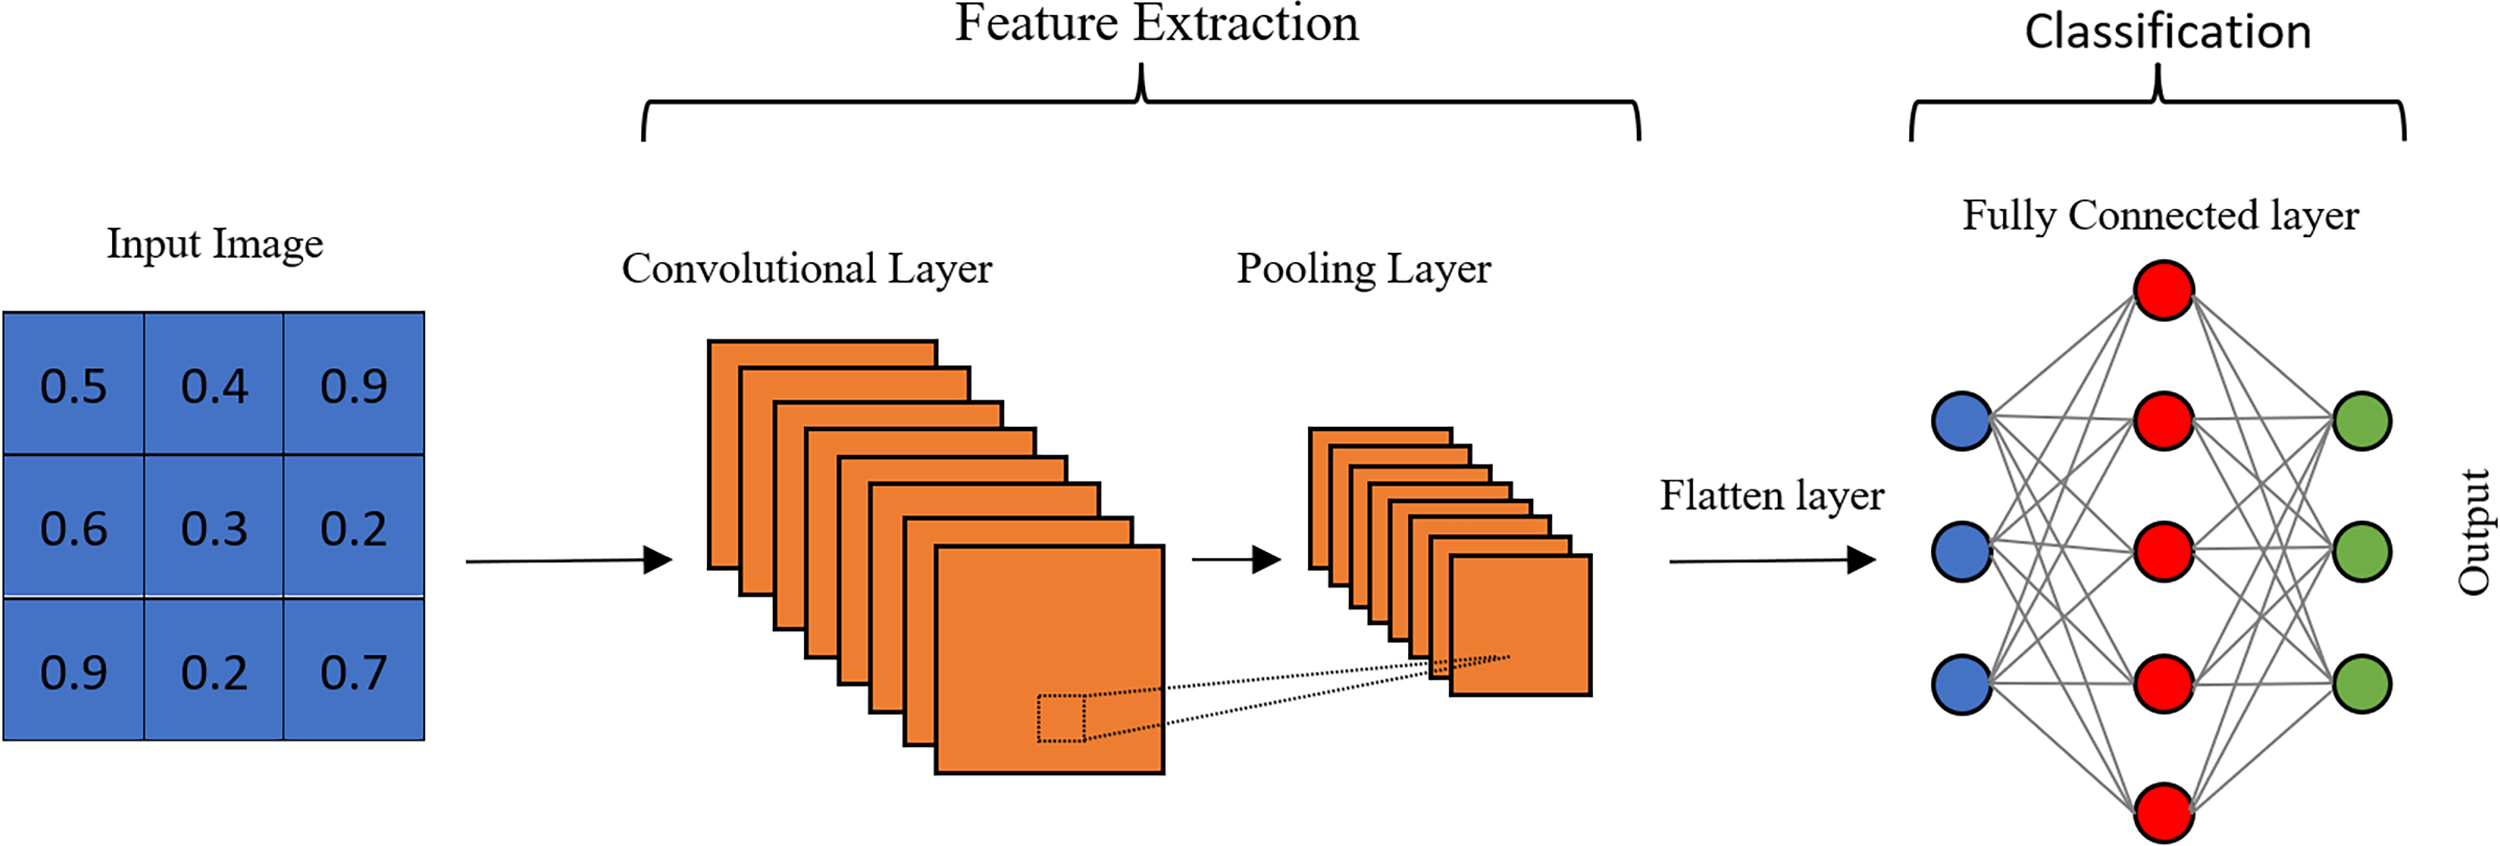
\includegraphics[width=0.5\textwidth]{CNNEXERCISE.png} 
    \caption{Basic CNN Architecture. The input image is passed through convolutional and pooling layers for feature extraction, followed by fully connected layers for classification.}
    \label{fig:cnn_overview}
\end{figure}

\subsection{\textbf{My CNN implementations with explanation}}
\subsubsection{\textbf{Initial Approach: CNN for CIFAR-10}}
\paragraph{\textbf{Explanation of the CNN Architecture}}
For my first CNN model, I again as previously with MLP created a network to classify images from the CIFAR-10 dataset. Below, I explain the structure of the CNN and how each part works:

\begin{itemize}
    \item \textbf{Convolutional Layers:}
    \begin{itemize}
        \item These layers use small grids of numbers called \textbf{filters} to scan the image. Filters detect patterns like edges or textures. 
        \item Each filter creates an output called a \textbf{feature map}, which shows where the pattern appears in the image.
        \item The model starts with two convolutional layers, each using 32 filters of size \(3 \times 3\). The \textbf{ReLU activation function} is applied after each convolution to keep only positive values. This helps the model learn better.
    \end{itemize}
    
    \item \textbf{Batch Normalization:}
    \begin{itemize}
        \item This step adjusts the output of the convolutional layer so that it has a mean of 0 and a standard deviation of 1. 
        \item This makes the training faster and more stable.
    \end{itemize}
    
    \item \textbf{Pooling and Dropout:}
    \begin{itemize}
        \item A \textbf{MaxPooling layer} reduces the size of the feature map by taking the largest value in small regions (e.g., \(2 \times 2\)). This keeps important information while making the data smaller and faster to process.
        \item \textbf{Dropout layers} randomly turn off some neurons (connections) during training to prevent overfitting. This ensures the model doesn’t rely too much on specific features and generalizes better to new data.
    \end{itemize}
    
    \item \textbf{Deeper Convolutional Layers:}
    \begin{itemize}
        \item Two more convolutional layers, each with 64 filters of size \(3 \times 3\), are added to detect more detailed patterns in the image.
        \item Batch normalization and MaxPooling are also applied to these layers, along with another dropout layer for regularization.
    \end{itemize}

    \item \textbf{Fully Connected Layers:}
    \begin{itemize}
        \item After the convolutional layers, the feature maps are \textbf{flattened} into a single long row of numbers.
        \item These numbers are passed through a \textbf{dense layer} with 256 neurons. A ReLU activation function is used again to learn patterns from the features.
        \item Another dropout layer with a 50\% rate is applied before the final layer to further reduce overfitting.
        \item The final layer has 10 neurons, one for each CIFAR-10 class, and uses the \textbf{softmax activation function} to produce probabilities for each class.
    \end{itemize}
\end{itemize}

\paragraph{\textbf{Training Process}}

The model was trained using the following settings:
\begin{itemize}
    \item \textbf{Optimizer:} The \textbf{Adam optimizer} was used to adjust the weights during training. It is faster and more efficient than traditional methods like simple gradient descent.
    \item \textbf{Loss Function:} The \textbf{categorical crossentropy} loss function measures how different the predicted probabilities are from the true labels. The goal is to minimize this loss during training.
    \item \textbf{Batch Size:} The data was processed in small groups of 32 images at a time (called batches) to make training efficient.
    \item \textbf{Epochs:} The model was trained for 60 complete passes through the dataset (called epochs).
\end{itemize}

\paragraph{\textbf{Results and Visualizations}}

Figure 10 shows how the model's accuracy and loss improved during training over 60 epochs. The model achieved a final test accuracy of approximately \textbf{\textit{0.8194}}. This demonstrates the model's ability to correctly classify most of the images.

\begin{figure}[h!]
    \centering
    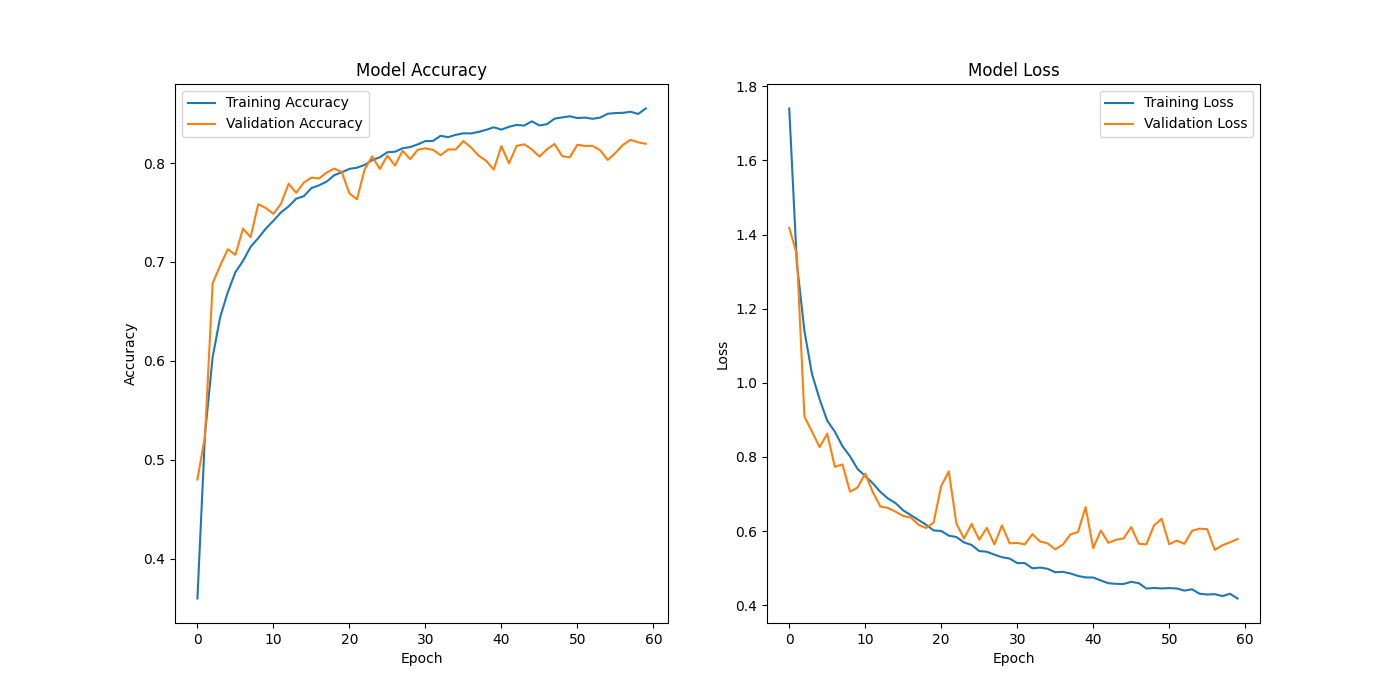
\includegraphics[width=0.5\textwidth]{training_history_CNN.png}
    \caption{Training and Validation Accuracy and Loss for the CNN Model.}
    \label{fig:cnn_training_history}
\end{figure}

To further evaluate the model, I visualized some examples of correctly and incorrectly classified images from the test set. Figure 11 shows 7 correct and 7 incorrect predictions.

\begin{figure}[h!]
    \centering
    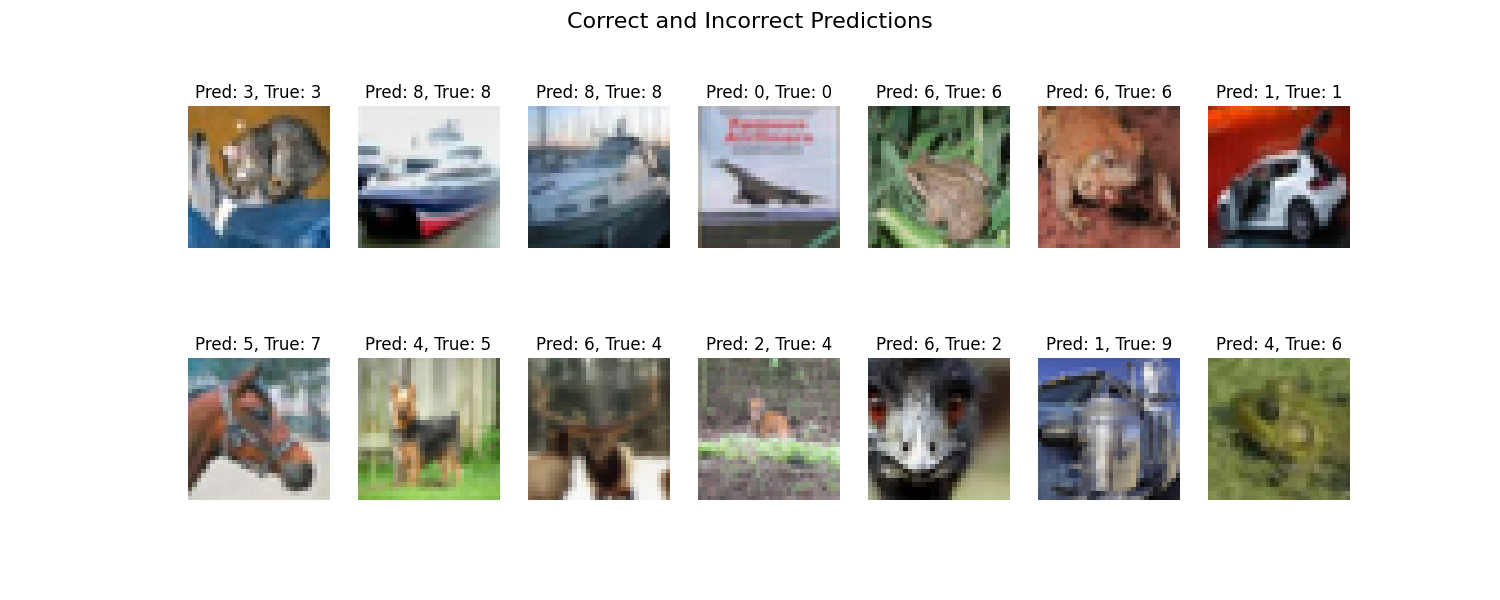
\includegraphics[width=0.5\textwidth]{sample_predictions_CNN.png}
    \caption{Examples of Correct and Incorrect Predictions for the CNN Model.}
    \label{fig:cnn_sample_predictions}
\end{figure}

\paragraph{\textbf{Observations}}

Some key takeaways from this CNN implementation are:
\begin{itemize}
    \item \textbf{Feature Extraction:} The convolutional layers effectively learned to detect patterns, which improved classification accuracy.
    \item \textbf{Regularization:} Dropout layers and batch normalization helped prevent overfitting and ensured the model worked well on new images.
    \item \textbf{Performance:} While the model performed well, adding more layers or data augmentation could further improve accuracy on complex images.
\end{itemize}

\subsubsection{\textbf{Enhanced Approach: CNN with Data Augmentation for CIFAR-10}}

\paragraph{\textbf{Explanation of the CNN Architecture}}

In this model, I extended the previous CNN architecture with a few enhancements:
\begin{itemize}
    \item Two convolutional layers with 32 filters followed by another two layers with 64 filters were used for feature extraction, as in the earlier model.
    \item A larger dense layer with 512 neurons was added before the output layer for better feature learning.
    \item Higher dropout rates (up to 60\%) were used to reduce overfitting.
\end{itemize}

\paragraph{\textbf{Data Augmentation}}

A key difference in this model was the use of \textbf{data augmentation}. This technique creates variations of the training images to make the model more robust and improve generalization. The augmentations applied include:
\begin{itemize}
    \item \textbf{Rotation:} Rotates the image randomly up to 10 degrees.
    \item \textbf{Shifting:} Shifts the image up or down, left or right by up to 10\% of its dimensions.
    \item \textbf{Shearing:} Applies a random shearing transformation.
    \item \textbf{Zooming:} Zooms into the image by up to 10\%.
    \item \textbf{Horizontal Flipping:} Flips the image horizontally.
\end{itemize}

These transformations helped the model learn to classify images under various conditions, improving its performance on unseen data.

\paragraph{\textbf{Training Process}}

The model was trained with the following setup:
\begin{itemize}
    \item \textbf{Data Generator:} A data generator applied augmentations during training, creating diverse inputs for the model.
    \item \textbf{Optimizer:} The RMSprop optimizer with a learning rate of 0.001 and a decay rate of \(1 \times 10^{-5}\).
    \item \textbf{Batch Size and Epochs:} A batch size of 128 and 100 training epochs were used.
\end{itemize}

\paragraph{\textbf{Results and Visualizations}}

Figure~\ref{fig:cnn_augmented_training_history} shows the training and validation accuracy and loss over 100 epochs. The model achieved a test accuracy of approximately \textbf{\textit{0.7916}}. Figure~\ref{fig:cnn_augmented_sample_predictions} shows some examples of correctly and incorrectly classified images.

\begin{figure}[h!]
    \centering
    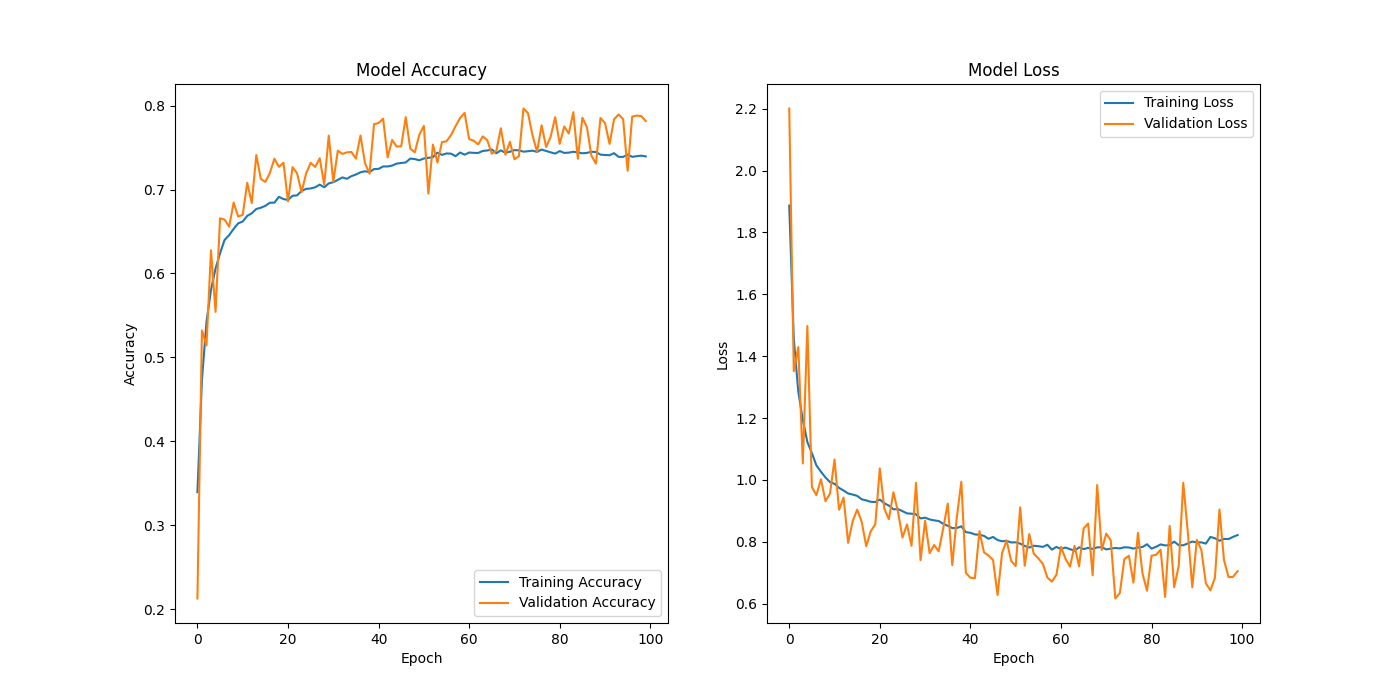
\includegraphics[width=0.5\textwidth]{training_history_CNN_Augmented.png}
    \caption{Training and Validation Accuracy and Loss for the CNN with Data Augmentation.}
    \label{fig:cnn_augmented_training_history}
\end{figure}

\begin{figure}[h!]
    \centering
    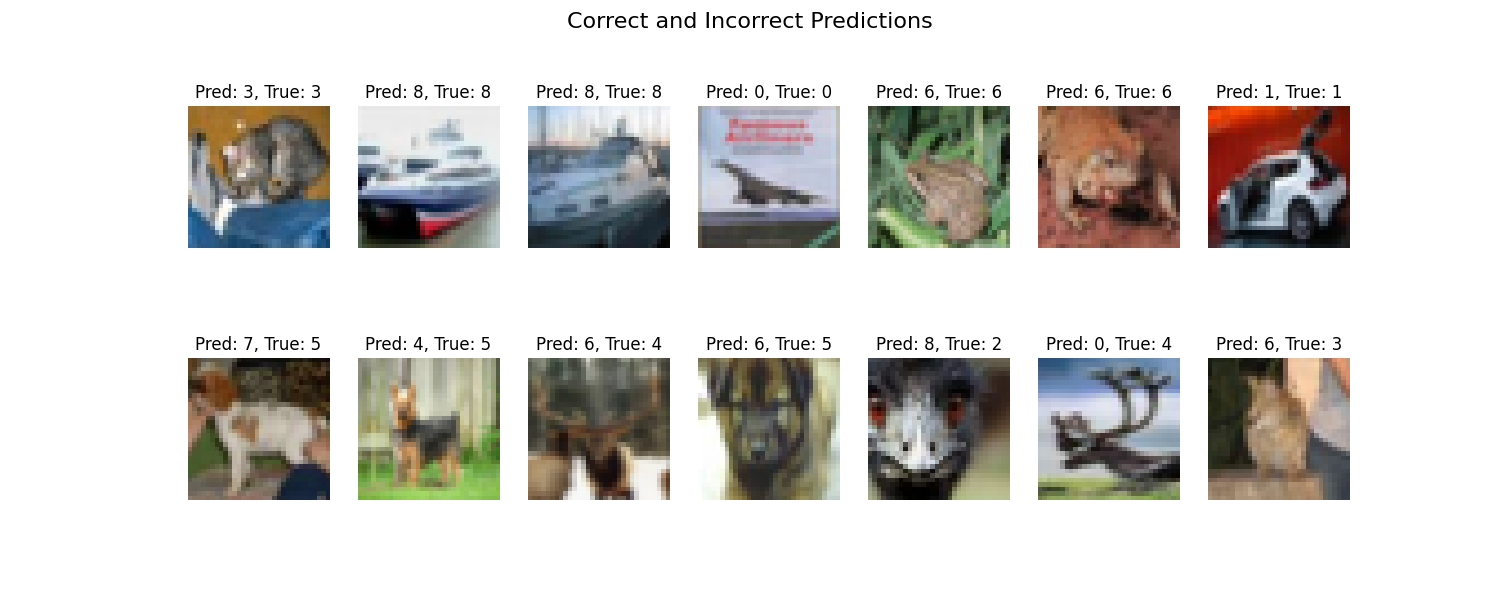
\includegraphics[width=0.5\textwidth]{sample_predictions_CNN_Augmented.png}
    \caption{Examples of Correct and Incorrect Predictions for the Augmented CNN Model.}
    \label{fig:cnn_augmented_sample_predictions}
\end{figure}

\paragraph{\textbf{Observations}}

Key differences and observations in this approach:
\begin{itemize}
    \item \textbf{Impact of Data Augmentation:} Augmentations made the model more robust to variations in input images, improving its generalization ability.
    \item \textbf{Lower Accuracy:} Compared to the previous CNN, this model did not perform as well as the non-augmented one.
    \item \textbf{Possible Risk of Overfitting:} Augmentation and higher dropout rates effectively could have portentially risen the risk of overfitting due to the higher complexity. We can also see that there are some minor fluctuations in validation metrics which are expected due to the higher data diversity.
    \item \textbf{Model converged earlier:} It didn't seem to need all 100 epochs to converge.
\end{itemize}


\section{References Section}
\begin{thebibliography}{1}
\bibliographystyle{IEEEtran}
\bibitem{ref1}
https://www.ibm.com/topics/knn
\bibitem{ref2}
https://www.geeksforgeeks.org/introduction-convolution-neural-network
\bibitem{ref3}
https://keras.io/api/layers
\bibitem{ref4}
https://elearning.auth.gr/mod/resource/view.php?id=89261
\bibitem{ref5}
https://keras.io/api/datasets/cifar10/
\bibitem{ref6}
https://www.cs.toronto.edu/~kriz/cifar.html
\end{thebibliography}

\end{document}


